% THIS DOCUMENT IS FOLLOWS THE VOLERE TEMPLATE BY Suzanne Robertson and James Robertson
% ONLY THE SECTION HEADINGS ARE PROVIDED
%
% Initial draft from https://github.com/Dieblich/volere
%
% Risks are removed because they are covered by the Hazard Analysis
\documentclass[12pt]{article}

\usepackage{booktabs}
\usepackage{tabularx}
\usepackage{hyperref}
\usepackage{array}
\usepackage{float}
\usepackage{graphicx}

\hypersetup{
    bookmarks=true,         % show bookmarks bar?
      colorlinks=true,      % false: boxed links; true: colored links
    linkcolor=red,          % color of internal links (change box color with linkbordercolor)
    citecolor=green,        % color of links to bibliography
    filecolor=magenta,      % color of file links
    urlcolor=cyan           % color of external links
}

\newcommand{\lips}{\textit{Insert your content here.}}

\input{../Comments}
\input{../Common}

\begin{document}

\title{Software Requirements Specification for \progname: subtitle describing software} 
\author{\authname}
\date{\today}
	
\maketitle

~\newpage

\pagenumbering{roman}

\tableofcontents

~\newpage

\section*{Revision History}

\begin{tabularx}{\textwidth}{p{3cm}p{2cm}X}
\toprule {\textbf{Date}} & {\textbf{Version}} & {\textbf{Notes}}\\
\midrule
Date 1 & 1.0 & Notes\\
Date 2 & 1.1 & Notes\\
\bottomrule
\end{tabularx}

~\\

~\newpage
\section{Purpose of the Project}
\subsection{User Business}
\lips
\subsection{Goals of the Project}
\lips
\section{Stakeholders}
\subsection{Client}
\lips
\subsection{Customer}
\lips
\subsection{Other Stakeholders}
\lips
\subsection{Hands-On Users of the Project}
\lips
\subsection{Personas}
\lips
\subsection{Priorities Assigned to Users}
\lips
\subsection{User Participation}
\lips
\subsection{Maintenance Users and Service Technicians}
\lips

\section{Mandated Constraints}
\subsection{Solution Constraints}
The system shall provide users access to their account and previous exercise information, provided a valid username and password.

\textbf{Justification}: User data stored in the user database is important to the account, but should be safely guarded without validation.\\

The system shall provide users with an overview of their exercises and data specific to individual exercises.

\textbf{Justification}: Users should be able to look back on their progress and see data on their exercises over time.\\

The system shall provide users the ability to upload video-feeds of them performing exercises, and return recommendations on their form.

\textbf{Justification}: The primary function of the system, users must be able to get form recommendations to assist in proper recovery and boost confidence in correct form. The system must be able to accept the video as input and be capable of returning relevant recommendations to the user.

\subsection{Implementation Environment of the Current System}
\begin{itemize}
  \item \textbf{Back End} (Processing): Source code written in Python.
  \item \textbf{Front End} (GUI): Source code written in platform specific application studio (EG. Android Studio).
  \item \textbf{OpenCV}: Library used to analyze user video-streams for required data.
  \item \textbf{Database}: Remotely accessible storage for user data.
\end{itemize}

\subsection{Partner or Collaborative Applications}
Physiotherapist scheduling, management, and patient-oriented softwares could be used in tandem, however the system is not designed with collaborative applications in mind.

\subsection{Off-the-Shelf Software}
\begin{itemize}
  \item \textbf{Database} software is previously implemented and simply interfaced by the system.
  \item \textbf{OpenCV} software is unmodified and only interfaced by the system.
\end{itemize}

\subsection{Anticipated Workplace Environment}
\begin{itemize}
  \item Physiotherapist patients in their residences or private spaces.
  \item Physiotherapists in their offices or assigned exercise spaces.
\end{itemize}

\subsection{Schedule Constraints}
As per the \href{https://github.com/M9Huynh/technically-functional/blob/7ff500c1d16686d4d7926d96109d83b87b307b87/docs/DevelopmentPlan/DevelopmentPlan.pdf}{Development Plan}:
\begin{itemize}
  \item Proof of Concept must be developed by November 17th, 2025.
  \begin{itemize}
    \item Demonstrations: November 17th - 28th.
  \end{itemize}
  \item Revision 0 must be developed by February 2nd, 2026.
  \begin{itemize}
    \item Demonstrations: February 2nd - 13th.
  \end{itemize}
  \item Revision 1 must be developed by March 23rd, 2026.
  \begin{itemize}
    \item Demonstrations: March 23rd - 29th.
  \end{itemize}
\end{itemize}

\subsection{Budget Constraints}
The development of the system must remain less than \$125 or the team begins paying out of pocket for development tools. Ideally the implementation remains free and open to use.

\subsection{Enterprise Constraints}
The system will attempt to mimic standards set by professional physiotherapists across Canada. Due to the nature of health care and physiotherapy market within Canada, the system will not provide medical care or medical assistance, simply wellbeing advice similar to that of a gym companion application.

\section{Naming Conventions and Terminology}
\subsection{Glossary of All Terms, Including Acronyms, Used by Stakeholders
involved in the Project}
\begin{table}[H]
\centering
\begin{tabular}{|l m{10cm}|}
  \hline
  \textbf{Term} & \textbf{Description} \\
  \hline \hline
  \textit{Flexion} & The act of contracting the muscles to bend the targeted joint, creating a smaller angle across the joint. \\ \hline
  \textit{Extension} & The act of contracting the muscles to unbend the targeted joint, creating a larger angle across the joint. \\ \hline
  \textit{Adduction} & The act of moving a part of the body towards the body’s midline. \\ \hline
  \textit{Abduction} & The act of moving a part of the body away from the body’s midline. \\ \hline
  \textit{Joint} & The connection between two bones which allows bending and movements of the limbs. In this document, this term mainly refers to the knee. \\ \hline
  \textit{Time Under Tension} & The time during an exercise where the targeted muscles are under strain. \\ \hline
  \textit{Range of Motion} or \textit{ROM} & The range of angles within which the user can move their joint from maximum stretching of the joint to maximum contraction of the joint. \\ \hline
  \textit{Form} & An all inclusive term referring to the position of body parts, their range of motion, and how they are coupled to execute the correct movement. \\ \hline
  \textit{Repetition} or \textit{Rep} & A single complete movement of an exercise from start to finish. \\ \hline
  \textit{Effectiveness} & Relevant to user-based goals to measure their own progress towards their recovery. (ie effectiveness in mobility increase, effectiveness in pain relief, etc.) \\ \hline
  \textit{Computer Vision} & The ability for the system to ‘see’ the user and extract relevant information. \\ \hline
  \textit{CI/CD} & Continuous integration/continuous deployment which automates building and limited testing of methods in our project. \\ \hline
\end{tabular}
\caption{Table of Project Terminology}
\end{table}

\begin{table}[H]
\centering
\begin{tabular}{|c l|}
  \hline
  \textbf{Acronym} & \textbf{Meaning} \\
  \hline
  A & Assumption \\
  PS & Physical System Description \\
  DD & Data Definition \\
  GD & General Definition \\
  GS & Goal Statement \\
  TM & Theoretical Model \\
  LC & Likely Change \\
  UC & Unlikely Change \\
  TUT & Time Under Tension \\
  DOF & Degrees of Freedom \\
  ROM & Range of Motion \\
  RMS & Root-Mean-Square (metric for error) \\
  Reps & Repetitions \\
  PTs & Physiotherapists \\
  FPS & Frame per Second \\
  CV & Computer Vision \\
  ML & Machine Learning \\
  FRs & Functional Requirements\\
  NFRs & Non-Functional Requirements \\
  PR & Pull Request \\
  SRS & Software Requirement Specification \\ \hline
\end{tabular}
\caption{Project Acronyms and Shorthands}
\end{table}

\section{Relevant Facts And Assumptions}
\subsection{Relevant Facts}
Relevant facts for this project are that about a third of patients needing physiotherapy can have improved efficacy due to their exertion and form factors. This leads to slower recovery or future injury later down the line. In some instances, this can lead to a permanent decrease in an affected joint’s range of motion and strength. Additionally, there is a gap from initially being prescribed the exercise and the accountability from doing exercises on the patients own time.

The primary target of this system is for patients of physiotherapists and physiotherapists.

\subsection{Business Rules}
Some business rules relevant to include that there will be a distinct user interface for general users of the application and a different user interface for physiotherapists. A patient must be directed to use the application from the physiotherapist and will have exercises assigned to  them on the system. Similarly, a physiotherapist can view and manage their patients but cannot access other patients outside their care.

A prescribed exercise chosen from the physiotherapist can have certain parameters and limitations, for example: sets, reps, frequency, etc. As well, the patient will be prompted after an exercise to give their perceived exertion as a result of the exercise on a scale of 1-10.

Furthermore, any data will not be shared without any explicit consent and will be stored securely.

\subsection{Assumptions}
\begin{table}[H]
\begin{tabular}{l m{10cm}}
  \textbf{\#} & \textbf{Assumption} \\
  A1 & The user of the system is a post-operative patient requiring physiotherapy. \\
  A2 & Users have prescribed physiotherapy exercises from a professional physiotherapist. \\
  A3 & Users prescribed exercise names will remain consistent across physiotherapists. \\
  A4 & Messages from the system are recommended actions and not healthcare advice. \\
  A5 & User’s smart devices will have an internet connection during video-feed uploading. \\
  A6 & User’s smart devices will be fully functional. \\
  A7 & User’s smart device camera will be fully functional. \\
  A8 & User’s smart device camera will be undamaged. \\
  A9 & User’s smart devices will meet or exceed the minimum system requirements. \\
  A10 & Users will have adequate space to record their exercises. \\
  A11 & Users will be able to read or listen to advice from the system during exercise video-feeds. \\
  A12 & Assume that the user knows how to use the smart device and generally how to navigate it when human-centered interfaces are used. \\
  A13 & Only one user is within the frame of the smart device. \\
  A14 & Users will be receptive to feedback.
\end{tabular}
\end{table}

\section{The Scope of the Work}
\subsection{The Current Situation}
Current at-home solutions for patients requiring physiotherapy, namely post-operative patients, are paid solutions that connect you to a physiotherapist to speak with or suggest to you a series of exercises based on some generically entered data. Patients are lacking a self-help tool to not only ensure they’re completing their exercises, but completing them correctly and safely as well.

Computer vision is being used in select places in the market to analyze form and give feedback, this exists for things like golf and tennis form analysis. However a stand-alone form-analyzing application which provides feedback independent of domain experts could scale far better and reach people who need it.

\subsection{The Context of the Work}
\begin{figure}[H]
  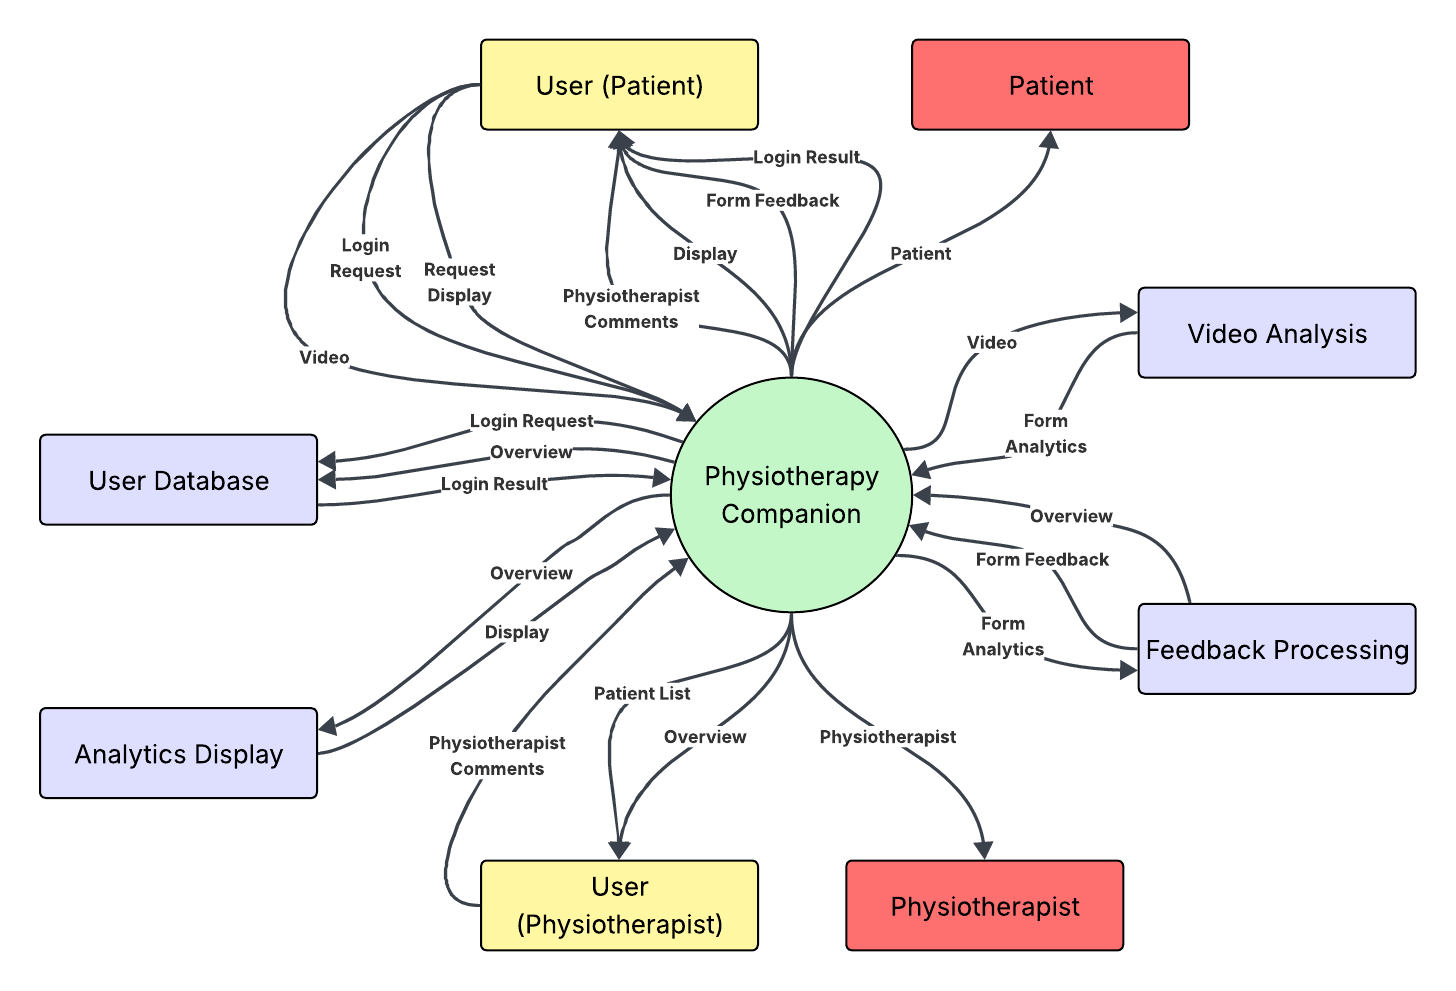
\includegraphics[width=\linewidth]{Context_Diagram.png}
  \caption{Work Context Diagram}
\end{figure}

\subsection{Work Partitioning}
\begin{table}[H]
\centering
\begin{tabular}{|m{3cm}|m{3cm}|m{8cm}|}
  \hline
  \textbf{Event} & \textbf{System Action} & \textbf{Description} \\ \hline
  User Requests Login & Login Request (in) & Compare user’s entered data with user database. \\ \hline
  Login Result Return & Login Result (out) & Return result, login or fail, to user based on data comparison. \\ \hline
  User Requests Display & Display Request (in) & Generate display with data from the user database. \\ \hline
  Display Return & Display Return (out) & Send the generated display to the user's GUI. \\ \hline
  User Submits Video & Form Feedback Request (in) & The user submits a video-feed for form analysis. \\ \hline
  Form Feedback Return & Form Feedback Return (out) & The system analyzes the form in the user’s video feed. The system generates form feedback and an overview from the analyzed information. The system generates a display with the newly added overview. The system sends the form feedback and the new display to the user. \\ \hline  
\end{tabular}
\caption{Work Partitioning}
\end{table}

\subsection{Specifying a Business Use Case (BUC)}
A user (patient) is prescribed exercises by a physiotherapist and uses the app to ensure they are doing the exercises correctly. This use case assumes the user is already logged in, and thus skips the login steps.

\begin{figure}[H]
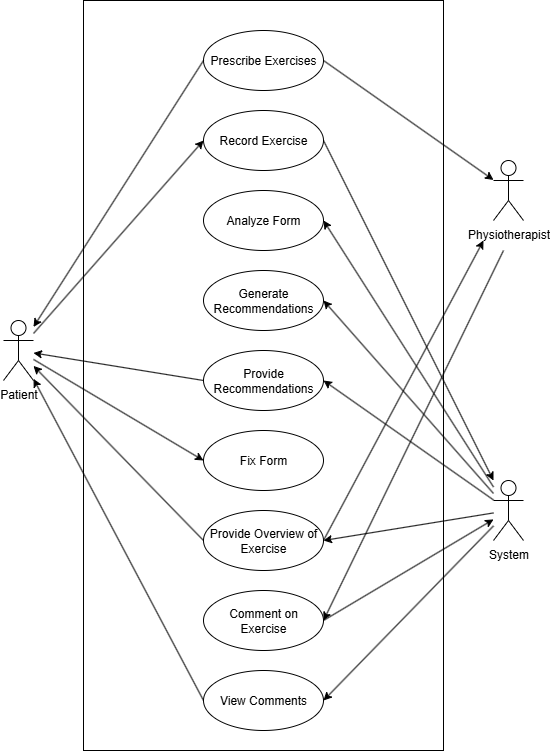
\includegraphics[width=\linewidth]{BUC.png}
\caption{Business Use Case Diagram}
\end{figure}

\section{Business Data Model and Data Dictionary}
\subsection{Business Data Model}
N/A 
This is not yet concrete, and will be fleshed out more at the implementation stage. Currently, the data flow should look very similar to that seen in the Work Context Diagram.

\subsection{Data Dictionary}
N/A
For the same reasons above, the data structures and specific metadata required for this section doesn’t yet exist within the project, and so cannot be entered here.

\section{The Scope of the Product}
\subsection{Product Boundary}
Refer to the Work Context Diagram for the boundaries of the system’s operations.
\subsection{Product Use Case Table}
\begin{figure}[H]
  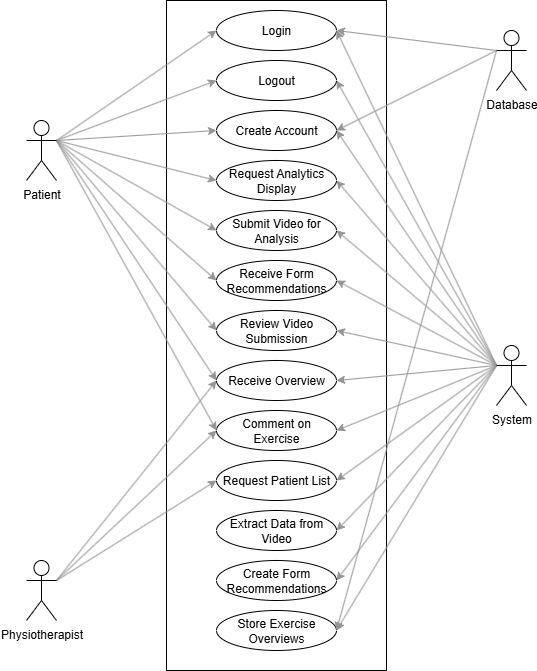
\includegraphics[width=13cm]{PUC.png}
  \caption{Product Use Case Table}
\end{figure}
\subsection{Individual Product Use Cases (PUC's)}
Where not specified, user is assumed to be user (patient).\\ \\
PUC1: Login\\
Event: User enters username and password and requests login.\\
Preconditions: User is not logged in.\\
Actors: User, System, Database\\
Normal Flow: User enters a valid username and password confirmed within the database and successfully accesses their pre-existing account.\\
Alternative Flow: User enters an invalid username and password which don’t verify in the database and the user is returned an error for invalid login information.\\ \\
PUC2: Logout\\
Event: User requests to logout of their account.\\
Preconditions: User is logged in.\\
Actors: User, System\\
Normal Flow: User requests to log out of their account. The system moves the user to the login page.\\
Alternative Flow: N/A\\ \\
PUC3: Create Account\\
Event: User requests to create an account.\\
Precondition: User is not logged in.\\
Actors: User, System, Database\\
Normal Flow: User enters an email, username, and password combination not already contained within the database. Email and username must be unique. The system creates an account for the user, stores the account information in the user database, and logs them into their account.\\
Alternative Flow: User enters an email or username that already exists within the user database, or a password which does not meet minimum requirements. The system returns an error and prompts the user to re-enter incorrect fields.\\ \\
PUC4: Request Analytics Display\\
Event: User refreshes analytics display (home page), user logs into their account, user returns to home page after an exercise.
Precondition: User is logged in and on the home page.\\
Actors: User, System\\
Normal Flow: After any of the events, the system uses all the stored user exercise overviews to refresh the analytics display.\\
Alternative Flow: If there are no stored exercise overviews for the user, the system prompts them to complete an exercise.\\ \\
PUC5: Submit Video for Analysis\\
Event: User submits a video-feed for form analysis.\\
Precondition: User is logged in and on the video submission screen.\\
Actors: User, System\\
Normal Flow: User submits a video-feed to the system for form analysis. The system accepts the video and recognizes the patient (user) within the video.\\
Alternative Flow: The system doesn’t recognize a patient within the video and prompts the user to fix any issues with their video-feed.\\ \\
PUC6: Receive Form Recommendations\\
Event: User is logged in and has submitted a video-feed for form analysis.\\
Precondition: User is logged in and the system has recognized them within the video-feed.\\
Actors: User, System\\
Normal Flow: System returns form recommendations based on data pulled from the video-feed and formulates the data into readable language recommendations which are displayed to the user.\\
Alternative Flow: System fails to draw analytical information from the video-feed and fails to create form recommendations for the patient (user).\\ \\
PUC7: Review Video Submission\\
Event: User has ended the video-feed upload.\\
Precondition: User is logged in, has submitted a video-feed for analysis, and has successfully received form recommendations.\\
Actors: User, System\\
Normal Flow: User can rewatch their video-feed submission with form recommendations in real-time before finally exiting the video submission screen.\\
Alternative Flow: User can cancel or request to redo their video-feed submission, taking them back to PUC5.\\ \\
PUC8: Receive Overview\\
Event: User has submitted and exited a video-feed submission.\\
Precondition: User has successfully submitted a video-feed submission, received recommendations, and exited the submission screen.\\
Actors: User (Patient), User (Physiotherapist), System\\
Normal Flow: System generates an overview of the exercise just submitted by the user and provides in natural language an overview to the user.\\
Alternative Flow: If the user didn’t submit their video-feed but exited and cancelled instead, no overview is created.\\ \\
PUC9: Comment on Exercise\\
Event: User creates a comment on an exercise.\\
Precondition: User (Patient) must be logged in and have completed one exercise, or, user (Physiotherapist) must be logged in and have at least one patient that has completed one exercise.\\
Actors: User (Patient), User (Physiotherapist), System\\
Normal Flow: User requests to create a comment on an exercise overview. User enters their own information into a text field and submits the comment. This comment is now visible to all users with access to that exercise overview.\\
Alternative Flow: User cancels their comment creation, and no comment is saved alongside the exercise overview.\\ \\
PUC10: Request Patient List\\
Event: User (Physiotherapist) requests or refreshes the patient list on their homepage.\\
Precondition: User (Physiotherapist) is logged in.\\
Actors: User (Physiotherapist), System\\
Normal Flow: System returns the list of all patients tied to the respective user (Physiotherapist) account, with access to their exercise overviews.\\
Alternative Flow: If the user (Physiotherapist) has no patients connected to their account, the system prompts them to add at least one patient.\\ \\
PUC11: Extract Data from Video\\
Event: System receives a video-feed from a user.\\
Precondition: User is recognizable in the video-feed.\\
Actors: System\\
Normal Flow: The system uses a CV library to extract necessary data relevant to the user’s form, storing the information locally for generating form recommendations, analytics displays, and overviews.\\ \\
PUC12: Create Form Recommendation\\
Event: System has extracted necessary form data from a video-feed.\\
Precondition: The video-feed was successfully analyzed by the CV library and received the necessary information.\\
Actors: System\\
Normal Flow: The system takes the form data and generates a naturally worded recommendation for the user’s form.\\ \\
PUC13: Store Exercise Overview\\
Event: Exercise overview has been created, comment has been submitted.\\
Precondition: Exercise overview or comment was successfully created, not cancelled.\\
Actors: System, Database\\
Normal Flow: The exercise overview is stored in the user database tied to the user’s account.\\

\subsection{System State Diagram}
\begin{figure}[H]
  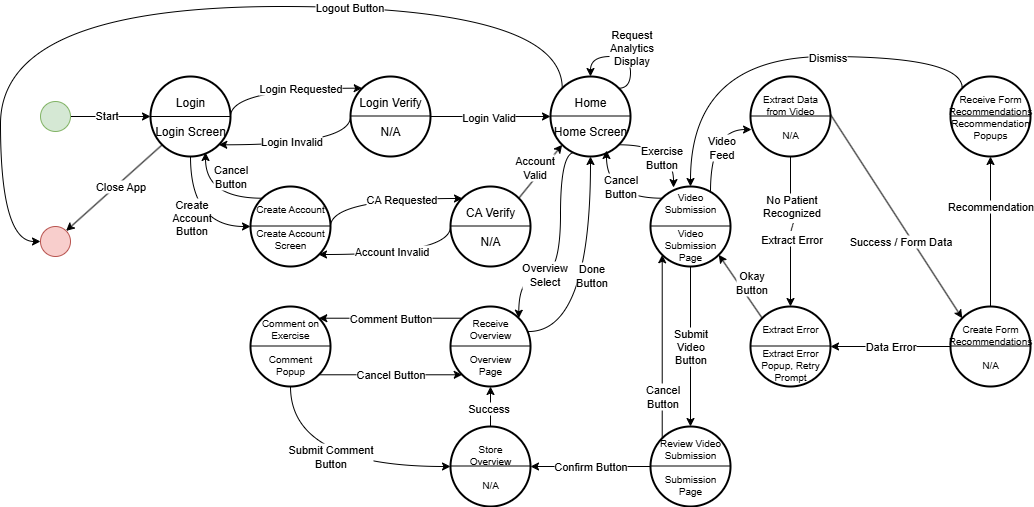
\includegraphics[width=\linewidth]{FSM.png}
  \caption{System State Diagram (State Machine)}
\end{figure}

\section{Functional Requirements}
\subsection{Functional Requirements}
\lips

\section{Look and Feel Requirements}
\subsection{Appearance Requirements}
\lips
\subsection{Style Requirements}
\lips

\section{Usability and Humanity Requirements}
\subsection{Ease of Use Requirements}
\lips
\subsection{Personalization and Internationalization Requirements}
\lips
\subsection{Learning Requirements}
\lips
\subsection{Understandability and Politeness Requirements}
\lips
\subsection{Accessibility Requirements}
\lips

\section{Performance Requirements}
\subsection{Speed and Latency Requirements}
\lips
\subsection{Safety-Critical Requirements}
\lips
\subsection{Precision or Accuracy Requirements}
\lips
\subsection{Robustness or Fault-Tolerance Requirements}
\lips
\subsection{Capacity Requirements}
\lips
\subsection{Scalability or Extensibility Requirements}
\lips
\subsection{Longevity Requirements}
\lips

\section{Operational and Environmental Requirements}
\subsection{Expected Physical Environment}
\lips
\subsection{Wider Environment Requirements}
\lips
\subsection{Requirements for Interfacing with Adjacent Systems}
\lips
\subsection{Productization Requirements}
\lips
\subsection{Release Requirements}
\lips

\section{Maintainability and Support Requirements}
\subsection{Maintenance Requirements}
\lips
\subsection{Supportability Requirements}
\lips
\subsection{Adaptability Requirements}
\lips

\section{Security Requirements}
\subsection{Access Requirements}
\lips
\subsection{Integrity Requirements}
\lips
\subsection{Privacy Requirements}
\lips
\subsection{Audit Requirements}
\lips
\subsection{Immunity Requirements}
\lips

\section{Cultural Requirements}
\subsection{Cultural Requirements}
\lips

\section{Compliance Requirements}
\subsection{Legal Requirements}
\lips
\subsection{Standards Compliance Requirements}
\lips

\section{Open Issues}
\lips

\section{Off-the-Shelf Solutions}
\subsection{Ready-Made Products}
Existing physiotherapy companion apps and other sport-specific or sports-medicine applications exist on the market, however they fail to do what this system intends. Existing physiotherapy companion apps either use human input on the other side of a submission, reducing scalability and increasing possibilities of human error. Some apps even require linking with hardware worn on the patient’s body to draw relevant form information for creating recommendations.

Existing form apps with computer-vision are used for very specific purposes, but not for physiotherapy recovery uses.

\subsection{Reusable Components}
The computer-vision aspects of form recommendation apps for sports, such as golf swings, tennis swings, or baseball batting practice, can be observed and mimicked for the computer-vision aspects of the application.

Some physiotherapy app systems that confirm users with physiotherapists, or confirm validity of physiotherapists, can also be mimicked to model the user database.

\subsection{Products That Can Be Copied}
There are no products that can be directly copied, but as mentioned in 20.2 there are parts of different existing applications that can be spliced to assist the implementation of the system.

\section{New Problems}
\subsection{Effects on the Current Environment}
\lips
\subsection{Effects on the Installed Systems}
\lips
\subsection{Potential User Problems}
\lips
\subsection{Limitations in the Anticipated Implementation Environment That May
Inhibit the New Product}
\lips
\subsection{Follow-Up Problems}
\lips

\section{Tasks}
\subsection{Project Planning}
\lips
\subsection{Planning of the Development Phases}
\lips

\section{Migration to the New Product}
\subsection{Requirements for Migration to the New Product}
As the system isn’t a migration from an older system, there are no changes needed to be made at a level any deeper than user onboarding. This means the requirements here are limited to onboarding patients in need of physiotherapy advice and physiotherapists who wish to ensure their patients are completing their exercises outside of appointments.
\subsection{Data That Has to be Modified or Translated for the New System}
N/A

As mentioned in 23.1, there is no change required on a level deeper than onboarding, this puts the data level out-of-scope for migration.


\section{Costs}
\lips
\section{User Documentation and Training}
\subsection{User Documentation Requirements}
Users, both patients and physiotherapists, will receive system prompts for next steps upon first usage of each of the system’s features. In addition to the prompts, first-time utilization will also come with help dialogue that lets the user know at a high level what the system is doing with inputs.

After first-time utilization, help buttons will remain to allow users to re-open this help dialogue if users are ever confused on system utilization.

\subsection{Training Requirements}
N/A

Users, both patients and physiotherapists, will learn all they need to through system prompts and help dialogue and will require no additional training to utilize the system.


\section{Waiting Room}
There are currently no updates planned to occur after the completion of the system outlined within this document. However, there are functionalities that would be pursued if the system was carried beyond the scope of this document.\\ \\
These additional features include, but are not limited to, the following:
\begin{itemize}
  \item Additional joints and exercises for physiotherapy advice and form recommendations.
  \item Additional security features such as two-factor authentication.
  \item Physiotherapist access to full-length patient video-streams (rather than just overview access).
  \item Advanced metrics and exercise information such as muscle activation.
\end{itemize}

\section{Ideas for Solution}
\lips

\newpage{}
\section*{Appendix --- Reflection}

\input{../Reflection.tex}

\input{../SRS_Reflection.tex}

\end{document}